%%%%%%%%%% Aquí va el código.
\subsection*{Pregunta 4.}
Considera el siguiente autómata
\begin{multicols}{2}
\begin{center}
  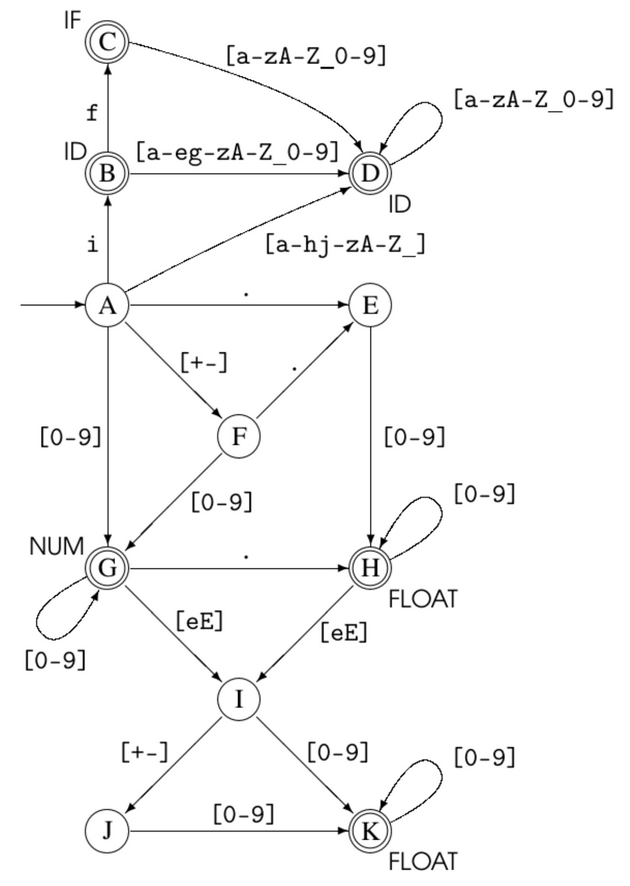
\includegraphics[scale=0.30]{./Automata.png}
\end{center}

\begin{itemize}
\item[$a$)] ¿Cuál es la definición del lenguaje que acepta este autómata?
  Proporciona la gramática regular de los tokens que se reconocen.
\item[$b$)] ¿Qué tokens son reconocidos al procesar la cadena 3e-z? Recuerda
  utilizar la técnica de la coincidencia más larga y si no es posible avanzar
  en un estado puedes hacer un retroceso o backtracking al estado de aceptación
  anterior para tratar de identificar el mayor número de tokens posible.
\end{itemize}
\end{multicols}
